\documentclass[officiallayout]{tktla} 
%\documentclass[officiallayout,a4frame]{tktla}
\usepackage[latin1]{inputenc}
\usepackage{latexsym}
\usepackage{graphicx}
\usepackage[]{algorithm2e}

% 
\usepackage{xargs}
\usepackage[colorinlistoftodos,prependcaption,textsize=tiny]{todonotes}
\newcommandx{\unsure}[2][1=]{\todo[linecolor=red,backgroundcolor=red!25,bordercolor=red,#1]{#2}}
\newcommandx{\change}[2][1=]{\todo[linecolor=blue,backgroundcolor=blue!25,bordercolor=blue,#1]{#2}}
\newcommandx{\info}[2][1=]{\todo[linecolor=OliveGreen,backgroundcolor=OliveGreen!25,bordercolor=OliveGreen,#1]{#2}}
\newcommandx{\improvement}[2][1=]{\todo[linecolor=red,backgroundcolor=red!25,bordercolor=red,#1]{#2}}
\newcommandx{\thiswillnotshow}[2][1=]{\todo[disable,#1]{#2}}
%


\title{Deep Learning Algorithms \\ for Control}
\author{Yuan Gao}
\authorcontact{gaoyuankidult@gmail.com\par
  http://www.cs.helsinki.fi/u/yuangao/}
\pubtime{September}{2015}
\reportno{0}
\isbnpaperback{000-00-0000-0}
\isbnpdf{000-00-0000-0}
\issn{1238-8645}
\printhouse{Unigrafia}
\pubpages{7} % --- remember to update this!
% For monographs, the number of the last page of the list of references
% For article-based theses, the number of the last page of the list of
% references of the preamble part + the total number of the pages of
% the original articles and interleaf pages.
\supervisorlist{Dorota Glowacka, University of Helsinki, Finland \newline  Leo K{\"a}rkk{\"a}inen, Nokia Research Center, Finland \newline Honkala Mikko Nokia Research Center, Finland}
\preexaminera{}
\preexaminerb{}
\opponent{}
\custos{}
\generalterms{}
\additionalkeywords{}
\crcshort{A.0, C.0.0}
\crclong{
\item[A.0] Example Category
\item[C.0.0] Another Example
}
\permissionnotice{
  To be presented in \ldots{} text of a long permission notice. Text of
  a long permission notice. Text of a long permission notice. Text of
  a long permission notice. Text of a long permission notice. Text of
  a long permission notice.
}

\newtheorem{theorem}{Theorem}[chapter]
\newenvironment{proof}{\noindent\textbf{Proof.} }{$\Box$}

\begin{document}

\frontmatter

\maketitle
\listoftodos
\begin{abstract}
Controlling a complicated mechanical system to perform a certain task, for example, making robot to dance, is a traditional problem studied in the area of control theory. Many successful applications like Google BigDog\cite{Raibert2008} and Google Self-driving car \todo{citation of self driving car} have been made in accordance to the new theories found in this field.

However more evidences show that in-cooperating with machine learning techniques in robotics can enable people to get rid of tedious engineering works of adjusting environmental parameters\todo{citation}. Many researchers like Jan Peters\todo{citation}, Sethu Vijayakumar, Stefan Schaal, Andrew Ng and Sebastian Thrun are the early explorers in this field. Based on the Partial Observable Markov Decision Process(POMDP) reinforcement learning, they contributed theory and practical implementation of several bench marks in this field.

Recently, one sub-field of machine learning called deep learning gained a lot of attention as a method attempting to model high-level abstractions by using model architectures composed by multiple non-linear layers. (for example \cite{Krizhevsky2012}). Several architectures of deep learning networks like deep belief network \cite{Hinton2006}, deep Boltzman machine \cite{Salakhutdinov2009}, convolutional neural network \cite{Krizhevsky2012} and deep de-noising auto-encoder \cite{Vincent2010} have shown its advantages in specific areas. Especially, convolutional neural network, which was invented by Krizhevsky, outperformed all the traditional feature-based machine learning techniques in ImageNet competition.

The main works of deep learning is more related to perception which deals with the problems like Sensor Fusion{OConnor2013}, Nature Language Processing(NLP)\cite{Cho2014} and Object Recognition\cite{Lenz2013}\cite{Hoffman2014}. Although considered briefly in J{\"u}rgen Schmidhuber's team\cite{Mayer2006}, the other area of robotics, namely control, remains more-or-less unexplored in the realm of deep learning.

There are two reasons about why these areas remain unexplored. The first reason is that deep learning method emphasizes on data driving techniques in which we need a lot of data to enable system to find important features whilst we don't have any dataset that can offer large amount of data. The second reason is that applying deep learning techniques requires introducing real robot platform to test the algorithm. This process is hard for researchers as they normally don't have resources for this complicated task.

The main focus of this thesis is to introduce general learning methods for robot control problem with an emphasize on deep learning method. As a consequence, this thesis tries to describe the transitional learning method as well as the emerging deep learning methods for robot control problem.

Ultimately, the author hope the readers of this thesis, even without much background in machine learning or robotics can understand the gists of solution for robot learning problems. \improvement{All paragraphs abstract needs to be rechecked.}
\end{abstract}

\begin{acknowledgements}
  This is a sample sentence that should look like normal text, and
  this is another. This is a sample sentence that should look like
  normal text, and this is another. This is a sample sentence that
  should look like normal text, and this is another.
\end{acknowledgements}

\tableofcontents

\mainmatter
\chapter{Introduction}

Controlling a complicated mechanical system to perform a certain task, for example making robot to dance, is a traditional problem studied in the field of control theory. Many successful applications like Google BigDog\cite{Raibert2008} and Google Self-driving car \cite{Guizzo2011a} have been made in accordance to the new theories found in this field.

However more evidences show that in-cooperating with machine learning techniques in robotics can enable people to get rid of tedious engineering works of adjusting environmental parameters\todo{citation}. Many researchers like Jan Peters\todo{citation}, Sethu Vijayakumar, Stefan Schaal, Andrew Ng and Sebastian Thrun are the early explorers in this field. Based on the Partial Observable Markov Decision Process(POMDP) reinforcement learning, they contributed first several algorithms enabling robot to learn to perform a certain task overtime.

Recently, one sub-field of machine learning called deep learning gained a lot of attention as a method attempting to model high-level abstractions by using model architectures composed by multiple non-linear layers. (for example \cite{Krizhevsky2012}). Several architectures of deep learning networks like deep belief network \cite{Hinton2006}, deep Boltzman machine \cite{Salakhutdinov2009}, convolutional neural network \cite{Krizhevsky2012} and deep de-noising auto-encoder \cite{Vincent2010} have shown its advantages in specific areas. Especially, convolutional neural network, which was invented by Krizhevsky, outperformed all the traditional feature-based machine learning techniques in ImageNet competition.

Based on the two trends we noticed, a natural path of research is to use deep learning methods for controlling movements of robot. Until the end of 2014,  the main works of deep learning are more related to a category of robotics called perception, which deals with problems like Sensor Fusion \cite{OConnor2013}, Nature Language Processing(NLP)\cite{Cho2014} and Object Recognition\cite{Lenz2013}\cite{Hoffman2014}. Although considered briefly in J{\"u}rgen Schmidhuber's team\cite{Mayer2006}, the other area of robotics, namely control, remains more-or-less unexplored in the realm of deep learning.

The researches done in J{\"u}rgen Schmidhuber's team provided several interesting structures that might be potentially useful for robot control. The name of one of these structures is called Long Short Term Memory (LSTM), which is one variation of Recurrent Neural Network(RNN). Several experiments like generating sequences\cite{Graves2013}, speech recognition\cite{Graves2013b} and neural turing machine \cite{Graves2014} show that it has ability of extracting and storing temporal information from data. As a consequence, this specific structure of RNN, with modification, can be applied for control problems of robots.

The main contribution of author is to invent a novel optimization method for system combining with POMDP reinforcement learning and LSTM.

There are two main focuses of this thesis. One main focus of this Thesis is to introduce general learning methods for robot control problem with an emphasize on deep learning method. this thesis tries to describe the transitional learning method as well as the emerging deep learning methods for robot control problem. Anther focus of this thesis is to introduce the main contribution of author in this field. With experiments, the author is able to show his own method can outperform the transitional machine learning methods of robot control problems.

\chapter{Reinforcement Learning}

If we would like to discuss what might be the most common way of learning, learning based on interacting with our environment is a natural idea to think about. When we were born in this world, we had no teachers around us. But tens of years passed, we learned to fear, to communicate with others and to write a paper. As a consequence, it is very natural to think that our environment is a great source of information. While playing around with environment, we learn by taking actions and getting reward from it. Now when we cook , when we do exercise, we are fully and acutely aware what will be the response of environment.

The RL is an area that studies the mechanism of the such kind of learning in a computational way. Generally the goal of RL is to find a way of mapping different states with different actions so that we could maximize the reward signals. 

There are two main approaches in area of reinforcement learning, one is based on Markov Decision Process(MDP)\cite{Sutton1998a}. Both methods have advantages and drawbacks when applied to robotics, another one is recurrent neural network(RNN)\cite{williams1989learning}.

In the following sections of this chapter, we may consider robot as an agent in all description of related techniques.

\section{Markov Decision Process}
Markov Decision Process (MDP) is a discrete time stochastic control process. We may consider a robot in a state $s$ of discrete state space $S$. The robot can take an action $a$ in all possible action set $A$ resulting in a state $s'$ . We can denote this process as transition function
$P_a(s, s')$ meaning the probability of moving from state
$s$ to state $s'$ through action a. Then after the robot executes action $a$ and results in $s'$ , it will receive a reward $r$ according to reward function denoted as $R_a(s, s ')$. The goal of reinforcement learning is to optimize cumulative reward of whole process. 

The problems of MDP is more clear to researchers as it is based on mathematical formalizations. On one hand, MDP-based methods together with optimization methods such as Gradient Partially Observable Markov Decision Processes (GPOMDP), projection method or nature gradient are state-of-art in robot trajectory learning. On another hand, as data collected from robot is different from normal data, it was pointed out the MDP-based methods suffers several curses\cite{Kober2013}.
\begin{itemize}
\item Curse of Dimensionality
\item Curse of Real-World Samples
\item Curse of Under-Modeling and Model Uncertainty
\item Curse of Goal Specification
\end{itemize}
The data is normally high dimensional, continuous and erroneous data in robot systems. It is considered to be difficult questions to neglect these issues and it is also hard to specify the goal of system i.e. what robot needs to be at last.

\section{Partially Observable Markov Decision Process}
\section{Dynamic Programming}
\section{Reinforcement Learning Methods}
\subsection{Temporal Difference Learning}
\subsection{Q-Learning}
\subsection{Adaptive Heuristic Critic}
\subsection{Prioritised Sweeping}
\subsection{Policy Gradient Methods}

\section{Classification of the Regarded RL Problems}
\subsection{High-Dimensionality}
\subsection{Partial-Observability}
\subsection{Continuous State and Action Spaces}
\subsection{Data-Efficiency}

\chapter{Recurrent Neural Networks}
Recurrent Neural Network(RNN) is a special structure of neural network that has recurrent connections. In the following sections of this chapter, we are going to discuss the details of this model.
\section{Feedforward Neural Networks}
In year 1957, the simplest structure of neural network called Perceptron was introduce by Frank Rosenblatt in Conell's Aeronautical Laboratory. This model consists only one cell and multiple connections. Figure~\ref{proceptron} shows the basic structure of proceptron.
\begin{figure}[h!]

  \centering
    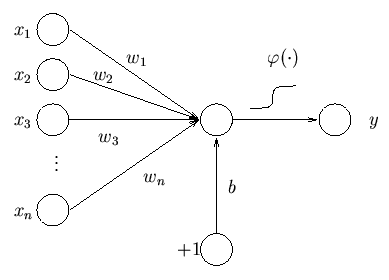
\includegraphics[width=0.5\textwidth]{proceptron}
  \caption{This picture shows the structure of Proceptron, the i'th input is shown as $X_i$ and corresponded weights are denoted as $w_i$. There is also a bias term name $b$ connected to cell, which, with a addition function, generates the output.}\label{proceptron}
\end{figure}

The formula of representing input and output is defined as:

\begin{equation}
y = \mathbf{w}\cdot\mathbf{x} + b
\end{equation}

If we consider $b$ also as one of the inputs, then the formula can be defined as:

\begin{equation}
y = \hat{\mathbf{w}}\hat{\cdot\mathbf{x}}
\end{equation}\label{pronceptron_formula}

where $ \hat{\mathbf{w}} = [\mathbf{w};b] $ and $\hat{\mathbf{x}} = [\mathbf{x};1]$.

This simple structure was considered promising initially from several points of view. But after further investigation, the Proceptron was proven that it can not classify many non-linear classes of patterns. However, its discovery leads to a field of research called neural networks in area artificial intelligence. As a consequence, since 1957, people started trying different methods for modifying this model to adapt to different problems. One important modification is to add a non-linear transformation function to the system i.e. after getting $y$ from Formula\ref{pronceptron_formula}, we use a function like tanh to get a new $\hat{y}$ to ensure the output is restricted in a range. Anther important modification of the system is to stack many proceptrons together to build a larger and complex model for the classification purpose. This kind of networks is normally called feed-forward neural networks as information send to this system is propagated only from lower layer to higher layer. Figure~\ref{feedforward_nn} shows the structure of feed-forward neural network system.

\begin{figure}[h!]
  \centering
    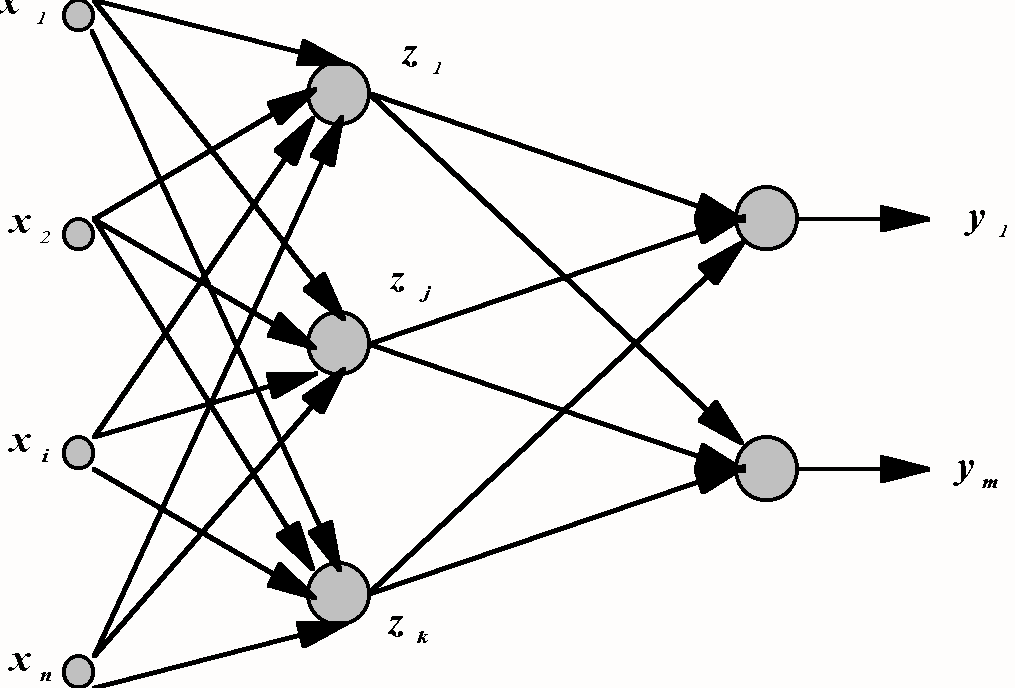
\includegraphics[width=0.7\textwidth]{feedforward_nn}
  \caption{This picture shows the structure of feedforward neural network. There are three layers in this network the input layer, hidden layer and the output layer. For connections from input layer to hidden layer, the i'th input is shown as $x_i$ and corresponded weights of hidden neuron $j$ is denoted as $W_{ij}$.}\label{feedforward_nn}
\end{figure}

The formula describing the each layer is then defined as:

\begin{equation}
\mathbf{o} = \sigma(W\mathbf{x})
\end{equation}
where $f(\cdot)$ is a non-linear transformation function.(e.g. tanh)

\section{Recurrent Neural Networks}
The Recurrent Neural Networks(RNN) contain at least one neuron that has at least one recurrent connection i.e. a connection that connects to itself or to lower layer. This special structure makes memory cell to be internal memory which enables network to memories the change of sequential data. Unlike the feed-forward neural network, the recurrent neural network is used for predicting next data point.

\begin{figure}[h!]
  \centering
    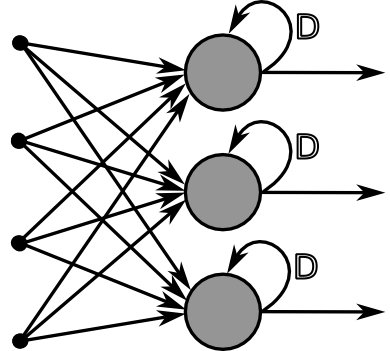
\includegraphics[width=0.5\textwidth]{recurrent_nn}
  \caption{This picture shows the structure of recurrent neural network. There are two layers in this networ namely input layer and hidden layer, the first layer contains notes connected to the input data. The second layer stores information and also forwards information to next layer. The cell in the hidden layer has a connection to itself which means the information stored in the cell at time $t-1$ also influences the information stored in the cell at time $t$}\label{feedforward_nn}
\end{figure}

\subsection{Finite Unfolding in Time}
When considering the structure of neural network, people normally application Finite Unfolding in Time for RNN. It means to introduce another dimension for RNN. In this way, the recurrent connection can be dealt with more easily.  In the following section, we will use a simple example for explaining this idea. The model we are going to use contains one input neuron, one hidden neuron and one output neuron. See Figure~\ref{simple_rnn} for reference.
\begin{figure}[h!]
  \centering
    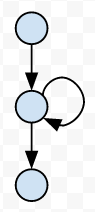
\includegraphics[width=0.2\textwidth]{simple_rnn}
  \caption{This picture shows the structure of a simple RNN. It contains three layers i.e. one input layer, one hidden layer and one output layer.}\label{simple_rnn}
\end{figure}
\change{This picture should be remade using tikz later}

In this figure, we mark input layer as $\mathbf{x}$, hidden layer as $\mathbf{s}$ and output layer as $\mathbf{o}$.

The basics idea of unfolding RNN in time is to copy RNN several times and connect them in a chronological order. If the connection is recurrent, then the connection should be connect to the same neuron of next time step.Figure~\ref{unfolded_simple_rnn} illustrates the model of unfolding simple RNN  for three time steps.

\begin{figure}[h!]
  \centering
    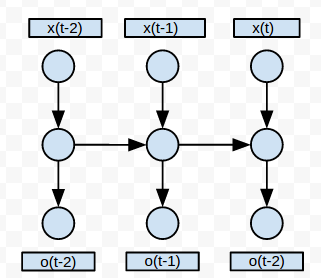
\includegraphics[width=0.5\textwidth]{unfolded_simple_rnn}
  \caption{This picture contains model that unfolds a simple RNN described in Figure\ref{simple_rnn} in three time steps. }\label{unfolded_simple_rnn}
\end{figure}
\change{This picture should be remade using tikz later}

The finite unfolding technique transforms a neural network with recurrent connection to a network that is easier to compute gradients. It is also easy for us to write this neural network's expression.

\begin{equation}
\mathbf{s_{t}} = \sigma(W\mathbf{x_t} + B\mathbf{s_{t-1}})
\end{equation}
Where $\mathbf{s_t}$ is the value of hidden state at time $t$ and $B$ is the weight matrix for updating hidden state information from time $t-1$ to $t$.


\subsection{Overshooting}
Considering that we only one time series, the task for RNN is to predict next data based on previous data we have. There are two steps for solving this problem. First we need to copy the data into two set and 

\subsection{Dynamical Consistency}
\section{Universal Approximation}
\subsection{Approximation by FFNN}

\subsection{Approximation by RNN}
\section{Training of RNN}

\subsection{Shared Weight Extended Backpropagation}

After getting data and designing the structure of network, the next important step is to train the network to model the data we have and also to predict next point in the data sequence. Training algorithm of recurrent neural network, called back-propagation, is introduced from feed-forward neural network. For simplicity of this algorithm, we consider a simple feed-forward neural network defined as:

\begin{equation}
y = \sigma(W\mathbf{x})
\end{equation}

where $W$ is a 3x4 matrix, $x$ is a vector of length 4 and $\sigma(\cdot)$ is an element-wise non-linear transformation.

This network only contains two layers including input layer and output layer. Input layer has four input neurons and output layer has three output neurons. The data we have is list of input-output pairs.

Formally the backpropagation algorithm is defined as :

\begin{algorithm}
 \KwData{List of input-output pairs }
 \KwResult{return the network}
 initialize network weights (often small random values)\;
 \While{training example ex}{
        prediction = neural-net-output(network, ex)
        actual = teacher-output(ex)\;
        compute error (prediction - actual) at the output units\;
        compute $\Delta W$ for all weights from hidden layer to input layer\;
        update network weights \;
        until all examples classified correctly or another stopping criterion satisfied
 }
 \caption{Backpropagation for two layers feed-forward neural network.}\label{backpropagation}
\end{algorithm}
\subsection{Learning Methods}
\subsection{Learning Long-Term Dependencies}

\section{Improved Model-Building with RNN} 
\subsection{Handling Data Noise} 
\subsection{Handling the Uncertainty of the Initial State}
\subsection{Optimal Weight Initialisation}

\chapter{Prior Arts of Combining RNN and RL}
\section{Neural Actor-Critic(idasi's group)}
\section{LSTM with POMDP objective function}
\section{PhD thesis, by Remi Coulom ?}

\section{DQN?}
\section{Hybrid Approch(RL with RNN)}
\section{Recurrent Models of Visual Attention?}       
\section{stanley gecco021 2002?}
\chapter{Experiment}
\section{RNN(LSTM) Implementation}
\section{Cart-pole Balancing Simulator}
\section{Learning a task of stacking wooden blocks}

This is a sample sentence that should look like normal text, and this
is another. This is a sample sentence that should look like normal
text, and this is another. This is a sample sentence that should look
like normal text, and this is another.


\begin{theorem}
This is a sample sentence that should look like normal text,
and this is another:
\[ y = x+3 \]
\end{theorem}

\begin{proof}
This is a sample sentence.
\end{proof}

\bibliography{library}
\bibliographystyle{siam}

\end{document}
